\documentclass{article}
\usepackage{assign}

\setcoursetitle{CS783: Visual Recognition}
\setassigncode{4}
\setauthname{Gurpreet Singh, Kamlesh Kumar Biloniya}
\setauthroll{150259, 160317}
\setheaddate{April 16, 2019}

\begin{document}
\makeheader

\begin{ssection}{Problem Statement}

	Our objective for this assignment was to semantically segment images in a completely unsupervised setting. The task to find objects without prior label information is challenging and is a major part of ongoing research in computer vision.

	We have been given an unlabeled dataset containing frames extracted surveillance videos. These images consist instances of multiple kinds of objects including cars, auto-rickshaws, pedestrians, etc. Given such an image, we need to produce a pixel-wise class prediction that segments the image into coherent clusters corresponding to objects (or instances of objects) in the image. We survey a number of well known, state of the art techniques, which are discussed in Section 2.
\end{ssection}

\begin{ssection}{Review}

	\begin{ssubsection}{W-net}

		The W-Net architecture \citep{wnet}, one of the state of the art architectures for image segmentation, ties two fully convolutional network (FCN) architectures (each similar to the U-Net architecture) together into a single autoencoder. The first FCN encodes an input image, using fully convolutional layers, into a K-way soft segmentation. The second FCN reverses this process, going from the segmentation layer back to a reconstructed image (see Figure \ref{fig:wnet}). The network is trained by jointly minimizing both the reconstruction error of the autoencoder as well as a “soft” normalized cut loss function on the encoding layer \citep{wnet}.

		\begin{figure*}[htpb]
			\centering
			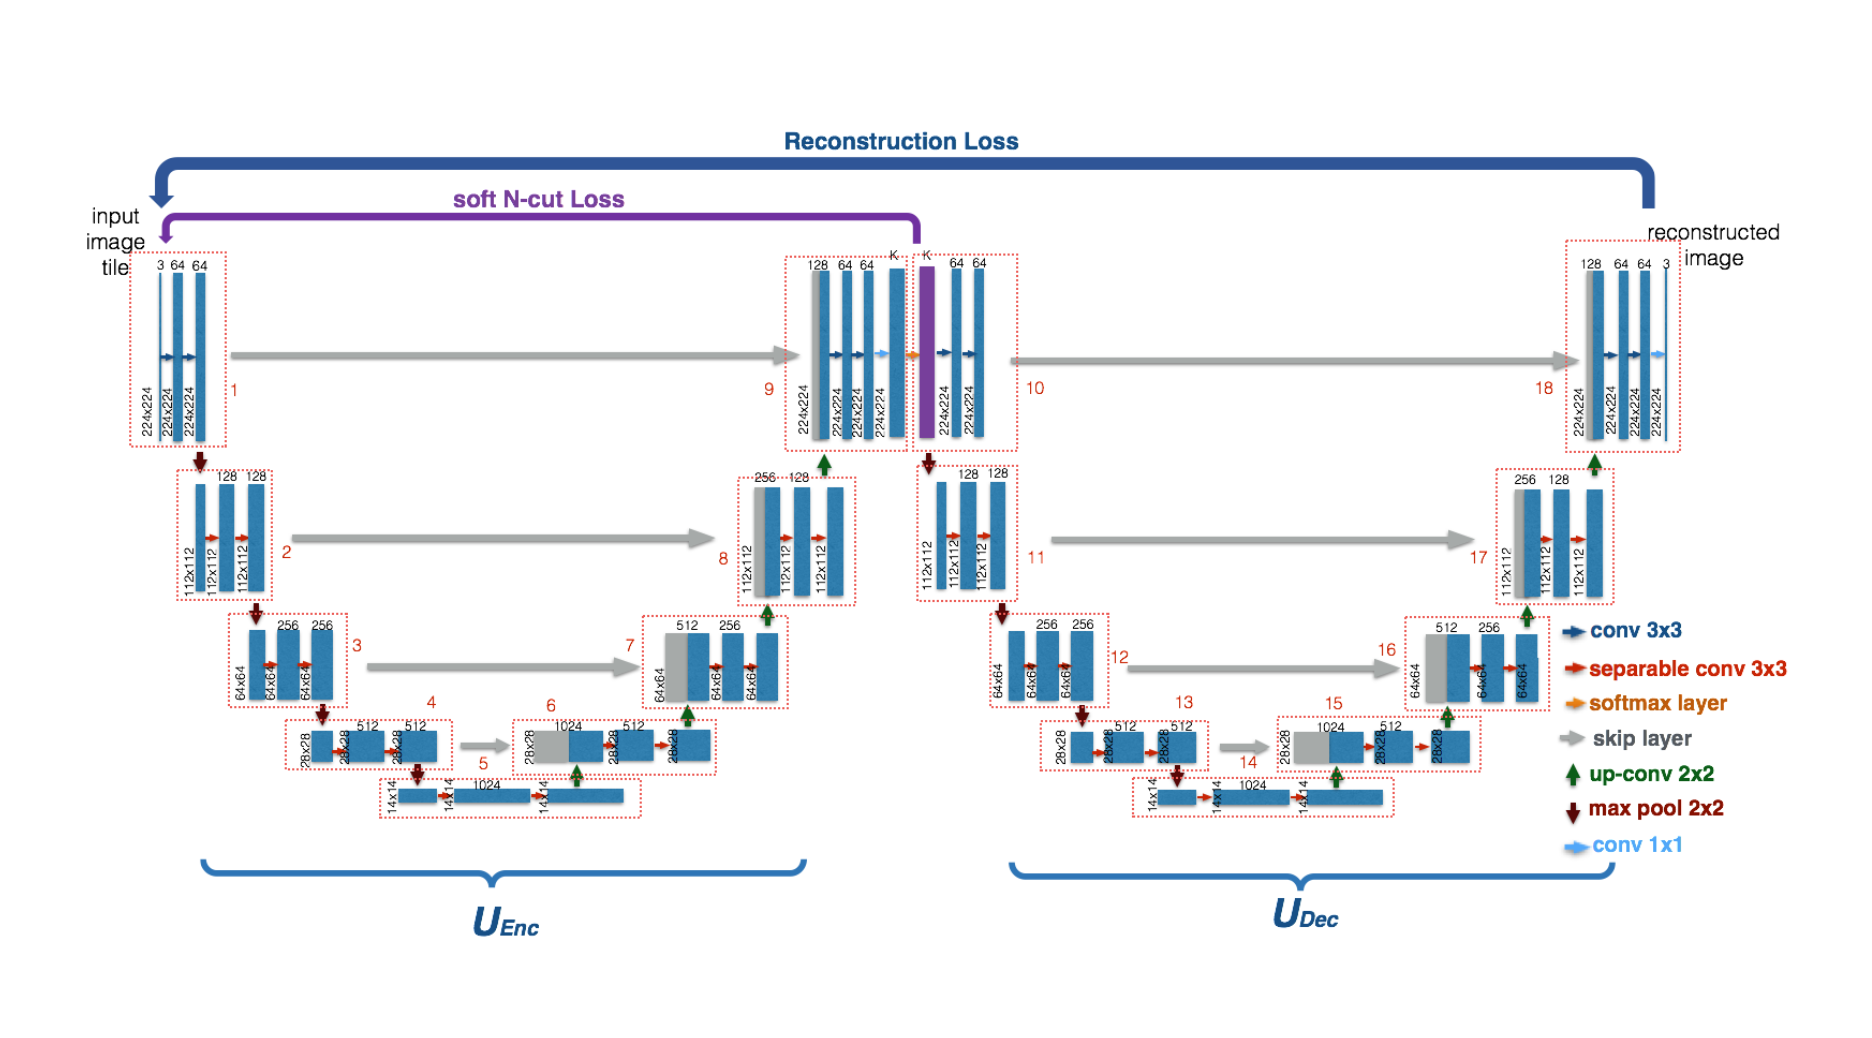
\includegraphics[width=0.8\linewidth]{includes/wnet-arch.png}
			\caption{W-Net architecture}
			\label{fig:wnet}
		\end{figure*}

		The problem with this architecture is that the image is over-segmented and therefore not properly representative of the image. In order to achieve state-of-the-art results, it further appropriately postprocess this initial segmentation in two steps: it first applies a fully conneceted conditional random field (CRF) smoothing on the outputted segments, and secondly the hierarchical segmentation method (by merging smaller segments) to obtain a final segmentation.

		Since the implementation of W-net is not straightforward, we used code from a github repository (\hyperlink{}{}), however it did not include the post-processing part and therefore we could not test the W-Net method properly. The results (before post-processing) are shown in Section 4.

	\end{ssubsection}

	\begin{ssubsection}{Unsupervised Image Segmentation using Backpropogation}

		\cite{backprop} proposed a simple method to semantically segment images using only a Convolution Neural Network to find pixel-wise cluster assignments. The idea is divided into three steps --
		\begin{enumerate}
			\item Use a segmentation technique such as SLIC to find superpixels/segments for the image.
			\item Build a CNN to compute pixel-wise feature vectors. Since we want feature-wise vectors, the network does not contain any pooling layers\footnote{It is actually possible to add pooling layers as long as we ensure to use Upconv layers to retain the original image size}. We, therefore, get feature vectors $\vx_n$ for each pixel $n$ in the image.
			\item Use a linear classifier to assign class/cluster to each pixel. Therefore, we obtain the response map $\set{\vy_n = \sW_c \vx_n + \vb_c}_{n = 1}^{N}$. This is implemented using a 1x1 conv layer as the purpose is to simply aggregate the channels into a $C$ sized layer where $C$ is the number of classes (fixed).
		\end{enumerate}

		Since we have a cluster assignment for each pixel, we are done. The training is based on the idea that each pixel in every superpixel should belong to the same cluster. Using this, \cite{backprop} propose the loss function as a cross-entropy loss between the pixel-wise soft-cluster assignments and the computed cluster assignment of the superpixel (computed by taking a mode of the predicted cluster assignments of each pixel in the superpixel).

		Although this method works well qualitatively, we observed a major issue with the approach. Since the loss function is simply a cross-entropy between predicted pixel assignments, the global optima would dictate all the pixels to be assigned the same cluster, as in that case the loss would be absolutely zero. The author avoid this issue using early stopping however this is not reliable and easily produce under-segmented images. We overcome this issue in our model which is explained in the next section.
	\end{ssubsection}

\end{ssection}

\begin{ssection}{Our Approach}

	We extend the method proposed by \cite{backprop} to fix the issues pointed out earlier. The reason the global optima assigns the same cluster to all pixels is because of lack of any terms bounding the cluster assignments to represent the pixels. In order to fix this, we changed the architecture to an Autoencoder which would ensure that the latent variables represent the pixel information by adding a reconstruction loss term. This is similar to other approaches such as the W-Net.

	The benefits of this approach are the simplicity, speed and efficiency of the model. One thing to note is that we can no longer use a classifier to assign clusters to pixels since any classifier can approach the optima by assigning the same cluster to all pixels. To overcome this, we consider the latent layer of the autoencoder to be our cluster assignments (after a softmax operation). This would ensure that the cluster assignments are coherent with the objects structure (because of the cross-entropy loss) and would make sure that the cluster assignments are representative of the pixels. The reconstruction loss, therefore, acts as a regularizer to our model.

	The final loss, to be precise, is now the sum of the cross-entropy loss between cluster assignments for each pixel with the cluster assignments of the superpixel and the reconstruction loss multiplied by a constant $\beta$ which acts as the regularization constant.

	To sum up, the encoder, which is a convolutional network, maps the input (e.g. an image) to acompact feature representation, and then the decoder, which is another convolutional network, reproduces the input from its lower-dimensional representation. The softmax of the feature representation acts as the soft-clustering assignment for each pixel, argmax of which would give us the most probable predicted cluster assignment.

	Same as W-Net, we observed the images to be somewhat over-segmented. Although originally we wanted to implement Hierarchical segmentation, however due to the shortage of time and complexity of the task, we could not do so. Instead, we prevent over-segmentation (upto an extent) by early stopping. This is possible because the encoder quickly trains itself to provide cluster assignments which would minimize the loss however the autoencoder trains rather slowly to fine-tune the cluster assignments.

	We also changed the SLIC method for image segmentation to Felzenszwalb's method. We observed much better results by making this change possibly owing to the fact that our model was over-segmenting the images. The difference between the segments generated using SLIC and Felzenszwalb's method are shown in Figure \ref{fig:segmentation}. This difference also made the code much faster since Felzenszwalb's method creates much fewer segments.

	\vspace{6mm}

	\begin{figure}[htpb]
		\centering
		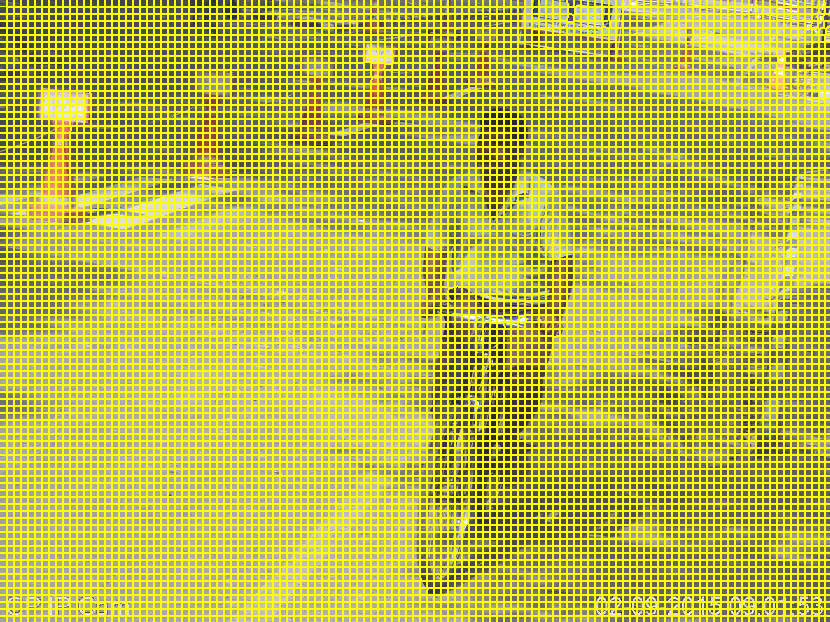
\includegraphics[width=0.4\textwidth]{includes/slic.png}
		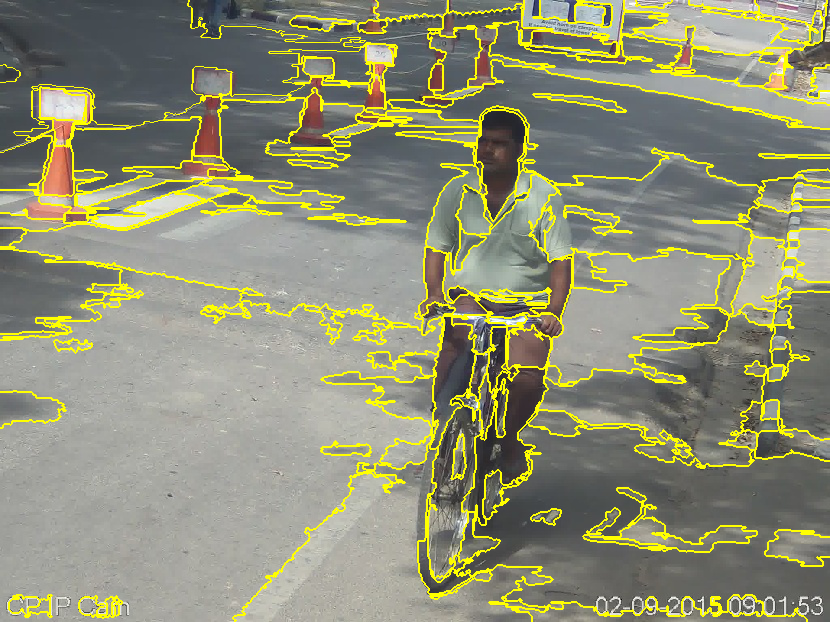
\includegraphics[width=0.4\textwidth]{includes/felzenszwalb.png}
		\caption{Segmentation using (left) SLIC and (right) Felzenszwalb's method of segmentation}
		\label{fig:segmentation}
	\end{figure}

\end{ssection}
\newpage

\begin{ssection}{Results}

	Since we do not have any labels, we only provide a qualitative analysis of the results obtained using the 3 methods (one being ours) discussed above. This comparison is given in Figure \ref{fig:comparison}

	\begin{figure}[htpb]
		\centering
		\begin{subfigure}[b]{0.4\textwidth}
		 	\centering
			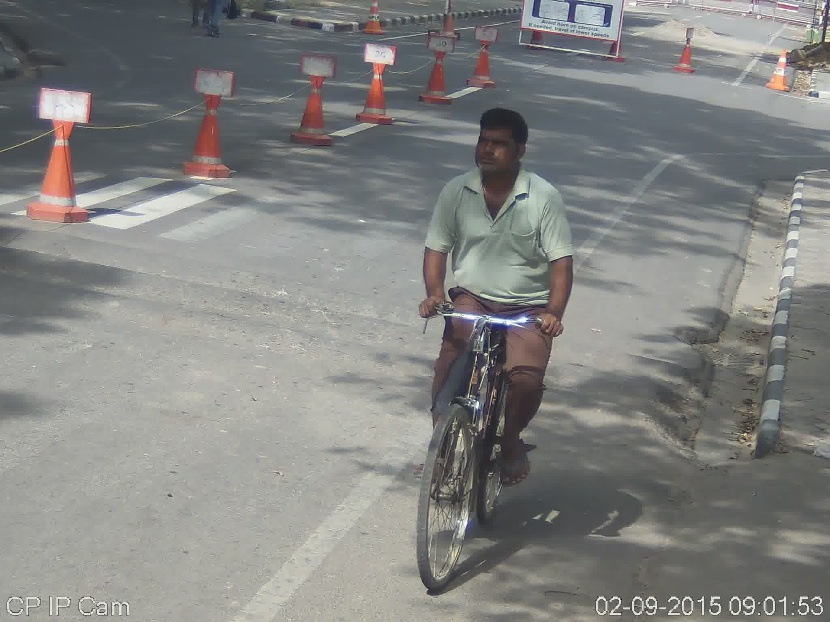
\includegraphics[width=\textwidth]{includes/original-image.png}
			\caption{Original Image}
		\end{subfigure}
		\begin{subfigure}[b]{0.4\textwidth}
		 	\centering
			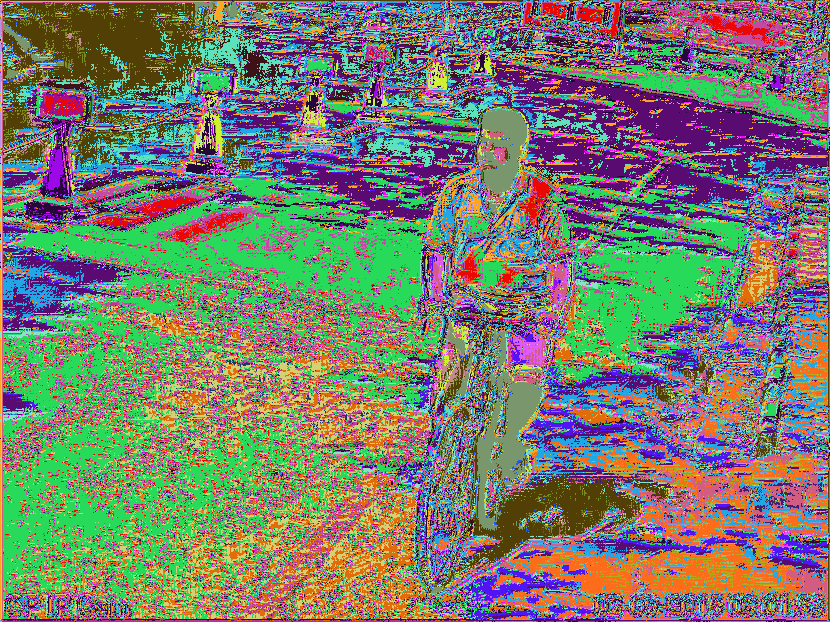
\includegraphics[width=\textwidth]{includes/wnet.png}
			\caption{Segmentation using W-Net}
		\end{subfigure}
		\begin{subfigure}[b]{0.4\textwidth}
		 	\centering
			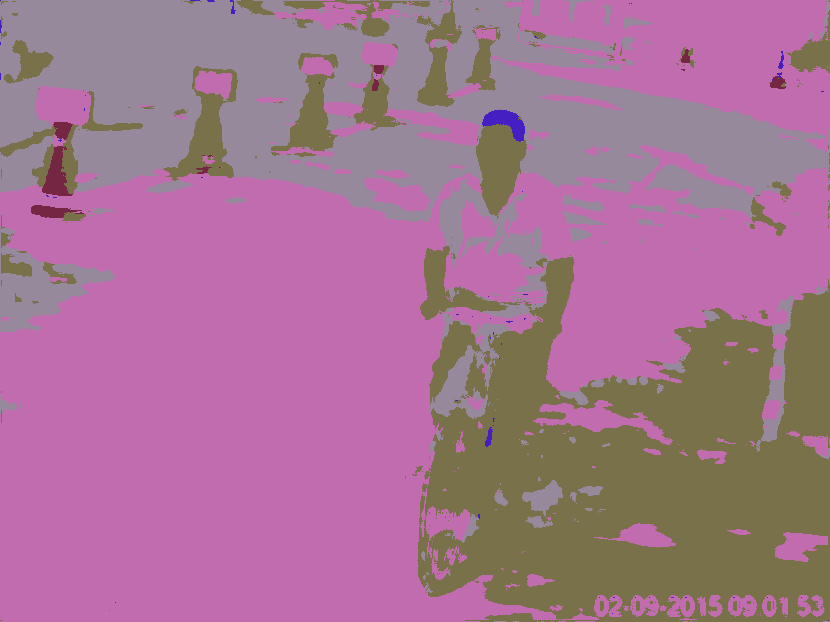
\includegraphics[width=\textwidth]{includes/backprop.png}
			\caption{Segmentation using Backpropogation}
		\end{subfigure}
		\begin{subfigure}[b]{0.4\textwidth}
		 	\centering
			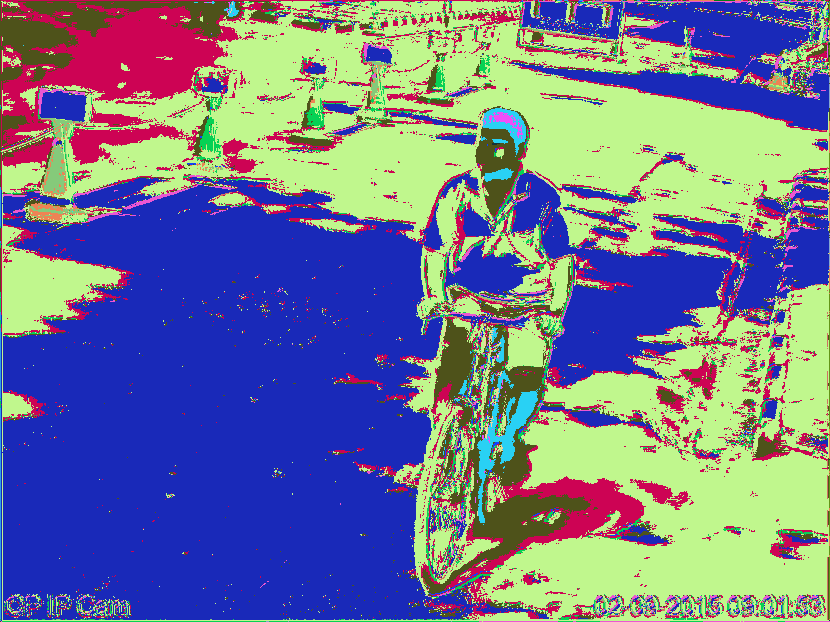
\includegraphics[width=\textwidth]{includes/ae-backprop.png}
			\caption{Segmentation using Our Approach}
		\end{subfigure}
		\caption{A Comparison of different methods for image segmentation}
		\label{fig:comparison}
	\end{figure}

	\vspace{5mm}

	\ditem{Problems with our Approach}

	As pointed out earlier, our approach over-segments the image. This is because of the cluster-assignments attempting to adapt to represent the pixel information. This can be avoided by using post-processing just as \cite{wnet} have used in W-Net.

	One problem is that edges are segmented separately. This, again, is because of the autoencoder loss. It is possible to fix this using C

	The advantages of using this approach over the method demonstrated by \cite{backprop} are the prevention of under-segmentation. Over W-Net, our model is faster, lighter and simpler to implement. Since the cross-entropy loss is much simpler and faster to compute than the Normalized Cut loss used by W-Net, our model is faster, though somewhat less efficient in reconstruction.

\end{ssection}

\bibliographystyle{plainnat}
\bibliography{references}

\end{document}
